% C.33 圆内接四边形 ABCD
\documentclass[tikz,border=4pt]{standalone}
\usepackage{ctex}
\usepackage{amsmath}
\usetikzlibrary{calc, arrows.meta}
\begin{document}
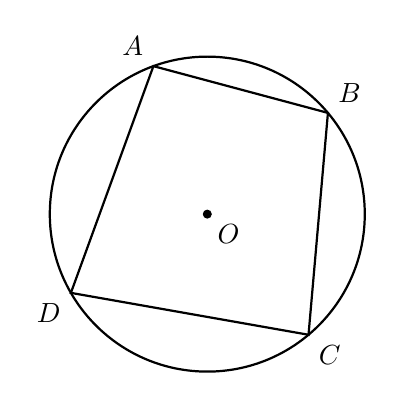
\begin{tikzpicture}[scale=1.0, thick]
  \coordinate (O) at (0,0);
  \draw (O) circle (2);
  \coordinate (A) at ({2*cos(110)},{2*sin(110)});
  \coordinate (B) at ({2*cos(40)},{2*sin(40)});
  \coordinate (C) at ({2*cos(-50)},{2*sin(-50)});
  \coordinate (D) at ({2*cos(-150)},{2*sin(-150)});
  \draw (A) -- (B) -- (C) -- (D) -- cycle;
  \filldraw (O) circle (1.2pt) node[below right] {$O$};
  \node[above left] at (A) {$A$};
  \node[above right] at (B) {$B$};
  \node[below right] at (C) {$C$};
  \node[below left] at (D) {$D$};
\end{tikzpicture}
\end{document}
